Nous avons implémenté deux extensions supplémentaires qui apportent des fonctionnalités supplémentaires mais aussi de la compléxité au système. C'est pourquoi nous avons les avons implémenté en parallèle et façon à ce qu'elles soient indépendantes entre elles.

\section{Gestion plus fine des ressources}

Il s'agit dans cette extension de permettre qu'une activité en cours d'exécution puisse être interrompue puis reprendre le cours de son exécution. Une telle interruption doit libérer les ressources utilisées par l'activité en question qui deviennent alors disponibles pour une autre activité. Pour une activité interrompue, sa reprise doit être permise à condition que les ressources dont il dépend soient disponibles.\\
Pour cette extension, il n'est pas nécessaire de modifier la structure du méta-modèle SimplePDL, ce qui implique qu'il n'y a pas de modification à apporter à l'outil de génération de syntaxe concrète textuelle, ni à l'outil de syntaxe concrète graphique. En effet, on agira principalement sur le réseau de Petri résultant de la transformation à partir d'un modèle SimplePDL. Nous allons donc adapter la requête de transformation SimplePDL vers PetriNet afin de permettre l'interruption et la reprise (soumise à condition) d'une activité.

\subsection{Transformation SimplePDL vers PetriNet}

Il est nécessaire de modifier le réseau de Petri mais tout en veillant à toujours respecter la spécification stipulant qu'une activité est soit :
\begin{itemize}
\item non commencée - \textit{Ready}
\item en cours - \textit{Started}
\item terminée - \textit{Finished}
\end{itemize}
Il ne faut donc pas supprimer les états déjà mis en place dans la partie précédente.\\

D'autre part, il est préférable de ne pas altérer le fonctionnement général du réseau de Petri engendré par la requête conçue dans la première partie afin de ne pas risquer une regression au niveau des fonctionnalités, particulièrement au niveau des observateurs associés à chaque activité. C'est pourquoi nous avons fait le choix de rajouter des places représentant deux sous états de l'état \textit{Started} :
\begin{itemize}
\item en cours d'exécution - \textit{Running}
\item interrompue - \textit{Interrupted}
\end{itemize}
Deux nouvelles transitions sont nécessaire pour permettre à une activité d'osciller entre ces deux sous états :
\begin{itemize}
\item interrompre - \textit{Interrupt} : \textit{Running} vers \textit{Interrupted}
\item reprendre - \textit{Resume} : \textit{Interrupted} vers \textit{Running}
\end{itemize}
On remarque que ces nouveaux sous états ne changent rien au fonctionnement des observateurs mis en place dans la première partie, cela permet de répondre à l'exigence qui précise que quelque soit le sous état dans lequel on se trouve (\textit{Running} ou \textit{Interrupted}), le temps continue à être décompté.\\

Pour cela, il faut donc générer de nouvelles places représentant ces sous-états dans la requête de transformation SimplePDL vers PetriNet, pour tous les éléments \textit{wd} de type \textit{WorkDefinition} parcourus dans le modèle SimplePDL en entrée :
\begin{verbatim}
p_running: petrinet!Place(
        name <- wd.name + '_running',
        marking <- 0,
        net <- wd.getProcess()),
p_interrupted: petrinet!Place(
        name <- wd.name + '_interrupted',
        marking <- 0,
        net <- wd.getProcess()),
\end{verbatim}

Il faut également insérer les transitions, toujours depuis le contexte des éléments de type \textit{WorkDefinition} :
\begin{verbatim}
t_interrupt: petrinet!Transition(
        name <- wd.name + '_interrupt',
        incomings <- a_r2i,
        outgoings <- a_i2i,
        min_time <- 0,
        max_time <- -1,
        net <- wd.getProcess()),
t_resume: petrinet!Transition(
        name <- wd.name + '_resume',
        incomings <- a_i2r,
        outgoings <- a_r2r,
        min_time <- 0,
        max_time <- -1,
        net <- wd.getProcess()),
\end{verbatim}

De même pour les arcs :
\begin{verbatim}
a_r2i: petrinet!Arc(
        source <- p_running,
        target <- t_interrupt,
        weight <- 1,
        kind <- #normal,
        net <- wd.getProcess()),
a_i2i: petrinet!Arc(
        source <- t_interrupt,
        target <- p_interrupted,
        weight <- 1,
        kind <- #normal,
        net <- wd.getProcess()),
a_i2r: petrinet!Arc(
        source <- p_interrupted,
        target <- t_resume,
        weight <- 1,
        kind <- #normal,
        net <- wd.getProcess()),
a_r2r: petrinet!Arc(
        source <- t_resume,
        target <- p_running,
        weight <- 1,
        kind <- #normal,
        net <- wd.getProcess()),
\end{verbatim}

Les arcs suivants sont nécessaires pour la libération lors de l'interruption d'une activité et pour la prise de ressources lors de la reprise du cours de son exécution d'une activité. Dans ce cas-là, on se positionne depuis le contexte des éléments \textit{ri} de type \textit{RessourceInstance} qui font le lien entre une activité (\textit{WorkDefinition}) et un type de ressource (\textit{RessourceDefinition}) et qui contiennent la donnée du nombre de ressources requises (qui seront libérées et reprises successivement) :

\begin{verbatim}
a_i2r: petrinet!Arc(
        source <- thisModule.resolveTemp(ri.activity, 't_interrupt'),
        target <- thisModule.resolveTemp(ri.type, 'p_ressource'),
        weight <- ri.instances,
        kind <- #normal,
        net <- ri.getProcess()),
a_r2r: petrinet!Arc(
        source <- thisModule.resolveTemp(ri.type, 'p_ressource'),
        target <- thisModule.resolveTemp(ri.activity, 't_resume'),
        weight <- ri.instances,
        kind <- #normal,
net <- ri.getProcess())
\end{verbatim}

Afin de ne pas perturber le système de gestion des ressources initial, il est nécessaire de préciser quelques spécifications supplémentaires :
\begin{itemize}
\item Une activité qui entre dans l'état \textit{Started}, entre par défaut dans le sous-état \textit{Running}
\item Pour pouvoir traverser la transition \textit{Finish} amenant à l'état \textit{Finished}, il faut être dans le sous-état \textit{Running} et évidemment dans l'état \textit{Started}
\end{itemize}

Cela implique le rajout les arcs suivants :
\begin{verbatim}
a_s2r: petrinet!Arc(
        source <- t_start,
        target <- p_running,
        weight <- 1,
        kind <- #normal,
        net <- wd.getProcess()),
a_r2f: petrinet!Arc(
        source <- p_running,
        target <- t_finish,
        weight <- 1,
        kind <- #normal,
        net <- wd.getProcess()),
\end{verbatim}

\subsection{Exemple d'exécution}

Dans cet exemple d'exécution, on vérifie que :
\begin{itemize}
\item si on est dans le sous-état \textit{Running}, les ressources sont prises et que l'on peut accéder aux transitions \textit{Finish} et \textit{Interrupt}
\item si on est dans le sous-état \textit{Interrupted}, les ressources sont libérées et que l'on peut accéder à la transition \textit{Resume} et pas à la transition \textit{Finish}\\
\end{itemize}

Vérifions ces propriétés, avec une exécution en cinq phases sur une même activité, correspondant aux cinq états suivants :
\begin{itemize}
\item \textit{Ready}
\item \textit{Started} \textit{Running}
\item \textit{Started} \textit{Interrupted}
\item \textit{Started} \textit{Running}
\item \textit{Finihed}
\end{itemize}

\subsection{Contraintes LTL}

Vérifier que si le processus est en \textit{Started}, toutes ses activités sont soit en \textit{Ready}, soit en \textit{Started}, soit en \textit{Finished}.

\section{Ressources alternatives}

Il s'agit ici de mettre en oeuvre une gestion alternative des ressources. Le principe est qu'il existe plusieurs configurations possibles de ressources.
Ainsi, soit une configuration A nécéssitant 2 machines et 3 développeurs et une configuration B avec 3 machines et 2 testeurs, on pourra exprimer le fait qu'une WorkDefition a besoin que la configuration A ou que la configuration B soit effective.

\subsection{Redéfinition du méta-modèle}

Il est donc clair que l'on doit modifier le méta-modèle pour expliciter cette possibilité de ``regroupement des ressources''.

\begin{figure}[!h] 
\begin{center}
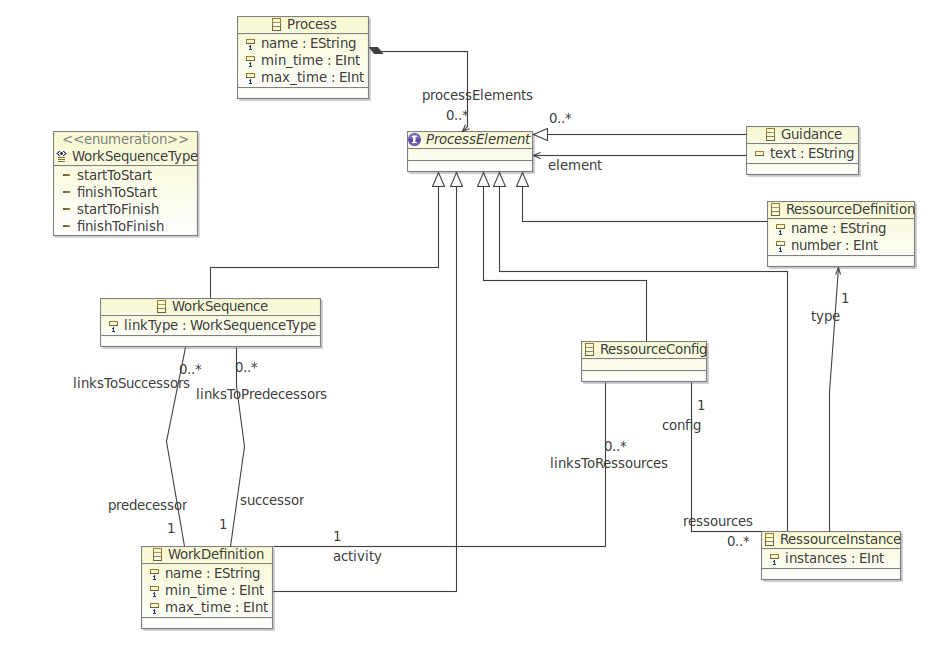
\includegraphics[width=15cm]{Capture-13.png}
\caption{Méta-modèle avec ressources alternatives} 
\label{img1} 
\end{center}
\end{figure} 

Et sous forme graphique,\\

\newpage

\begin{figure}[!h] 
\begin{center}
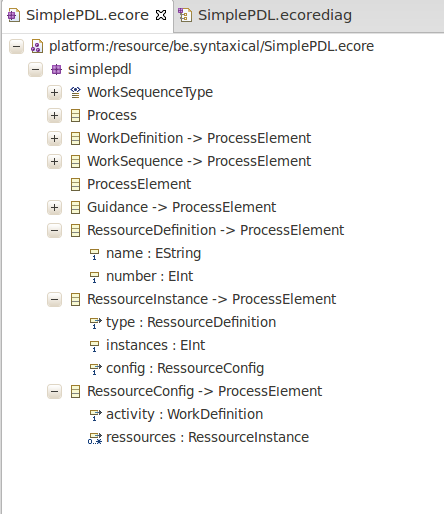
\includegraphics[width=8cm]{Capture-14.png}
\caption{Méta-modèle sous forme graphique} 
\label{img1} 
\end{center}
\end{figure} 

Pour permettre ce regroupement, on rajoute une classe RessourceConfig. Cette classe va contenir des liens vers des RessourceInstance. Ainsi, on va exprimer le fait qu'il peut exister plusieurs configurations mettant en oeuvre différents jeux de ressources.\\

On remplace donc le lien de WorkDefinition a RessourceInstance, par un lien de WorkDefinition a RessourceConfig. Ce lien a une multiplicité 0..\* car on peut avoir plusieurs Configurations pour une même WorkDefinition.

\subsection{Transformation SimplePDL vers PetriNet}

Prenons l'exemple suivant, 

\begin{figure}[!h] 
\begin{center}
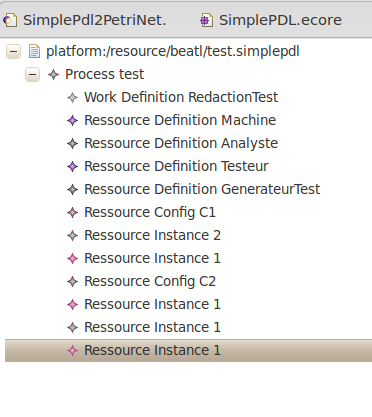
\includegraphics[width=8cm]{Capture-15.png}
\caption{Exemple mis en oeuvre} 
\label{img1} 
\end{center}
\end{figure}

On dispose de 4 ressources : Machine, Analyste, Testeur, GenerateurTest.
Par souci de lisibilité, on limite le nombre de WorkDefinition, à une seule : redactionTest. On définit également deux configurations C1 et C2. C1 met en oeuvre deux WorkInstance (Machine, 2) et (GenerateurTest,1). C2 met en oeuvre trois WorkInstance (Analyste,1), (GenerateurTest,1) et (Machine,1).\\

Cet exemple va nous permettre d'illustrer les transformations qui doivent être effectuées.\\

Il faut donc reprendre la transformation SimplePDL vers PetriNet et transformer la gestion des Ressources. Toujours par souci de lisibilité, on s'affranchit de la génération d'observateurs.\\

Le principe du réseau de pétri gérant la configuration des ressources est le suivant :\\

\begin{itemize}
\item Il est possible de choisir entre chacune des configurations (si du moins il y a suffisament de ressources)
\item Une fois que l'on a choisi de démarrer avec une configuratio, on ne pourra plus choisir l'autre
\item Les Ressources utilisées doivent être restituées à la fin de l'activité, et qui plus est dans la bonne configuration.
\end{itemize}

Il ressort de cette analyse que l'on va devoir utiliser des places nous indiquant :\\

\begin{itemize}
\item Quelle configuration est choisie : ConfigurationName\_used
\item Une configuration a été choisie : ProcessName\_ress\_l\\
\end{itemize}

Et des transitions pour :\\

\begin{itemize}
\item Choisir une configuration : ConfigurationName.start
\item Rendre les ressources : ConfigurationName.finished\\
\end{itemize}

Pour l'exemple cité précédement, on obtient donc le réseau de pétri suivant :\\

\begin{figure}[!h] 
\begin{center}
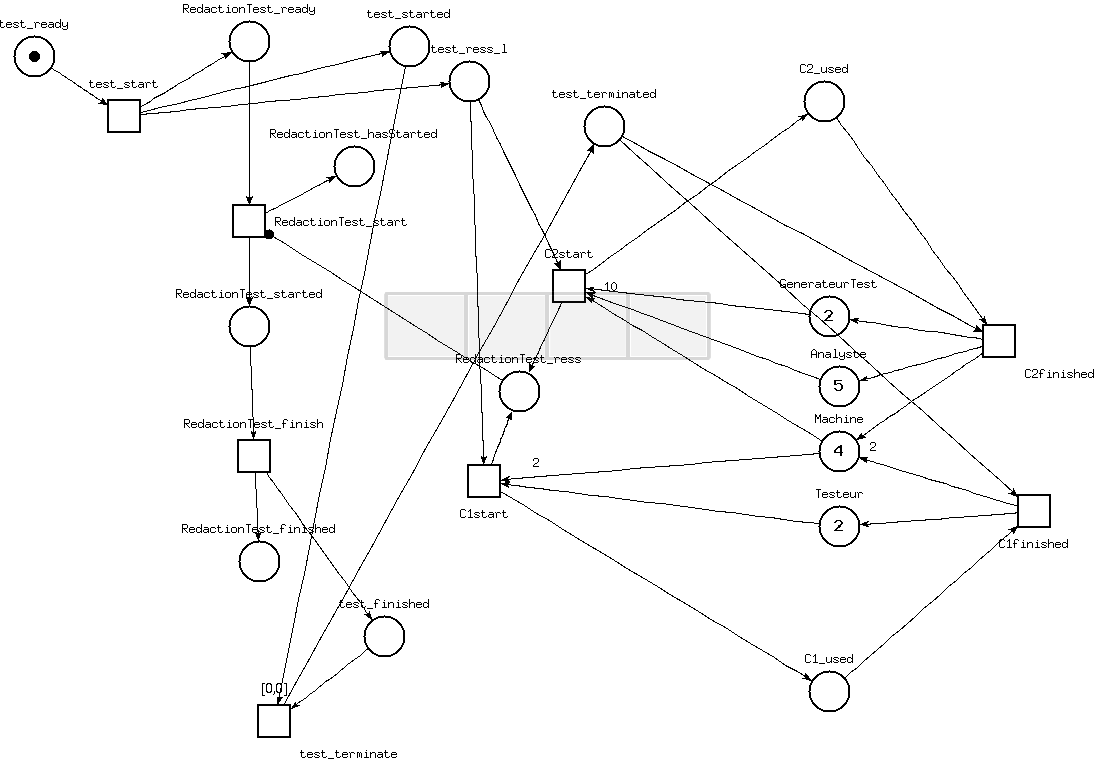
\includegraphics[width=15cm]{Capture-16.png}
\caption{Réseau de pétri obtenu} 
\label{img1} 
\end{center}
\end{figure}

Bien entendu, le code de la transformation a été adapté pour fornir ces changements. Il est disponible en annexe.\\

Pour ce qui est de la transformation PetriNet2Tina, il n'y a toujours aucune raison de la modifier car, on a pu conserver la même structure pour le méta-modèle PetriNet.ecore.\\







